\documentclass{VUMIFPSkursinis}
\usepackage{algorithmicx}
\usepackage{algorithm}
\usepackage{algpseudocode}
\usepackage{amsfonts}
\usepackage{amsmath}
\usepackage{bm}
\usepackage{caption}
\usepackage{color}
\usepackage{float}
\usepackage{graphicx}
\usepackage{listings}
\usepackage{subfig}
\usepackage{wrapfig}
\usepackage{multirow}
\usepackage{longtable}
\usepackage{array,makecell}

% Titulinio aprašas
\university{Vilniaus universitetas}
\faculty{Matematikos ir informatikos fakultetas}
\department{Programų sistemų katedra}
\papertype{Programų sistemų inžinerija: 1 laboratorinis darbas}
\title{Stalo žaidimų programėlė}
\titleineng{Board Games Application}
\status{2 kurso 5 grupės studentai}
\author{Elena Reivytytė}
\secondauthor{Matas Šilinskas}
\thirdauthor{Kasparas Taminskas}
\fourthauthor{Aidas Vaikšnoras}
\fifthauthor{Tadas Žaliauskas}
\supervisor{dr. Vytautas Valaitis}
\date{Vilnius – \the\year}

% Nustatymai
% \setmainfont{Palemonas}   % Pakeisti teksto šriftą į Palemonas (turi būti įdiegtas sistemoje)
\bibliography{bibliografija}

\begin{document}
\maketitle

\sectionnonum{Anotacija}
Šis 2-ojo laboratorinio darbo dokumentas yra skirtas aprašyti stalo žaidimų mobiliosios programėlės reikalavimų specifikacijai. Dokumente išdėstomi pagrindiniai sistemos reikalavimai, kurie formuluojami po dalykinės verslo srities analizės jau turint konkretesnį kuriamos sistemos poreikių sąrašą.

\tableofcontents

\sectionnonum{Įvadas}
\textbf{Dalykinė sritis:} stalo žaidimai

\textbf{Probleminė sritis:} siekiama išspręsti stalo žaidimų žaidėjų skaičiaus trūkumo realiame pasaulyje problemą.

Programėlės vartotojai: 
\begin{itemize}
	\item Stalo žaidimų mėgėjai
	\item Stalo žaidimų kūrimo kompanijos
\end{itemize}

Stalo žaidimų mobilioji programėlė yra projektas, skirtas išnaudoti dar neužpildytą nišą mobiliųjų programėlių versle, sukuriant nemokamą, reklama pagrįstą programėlę, skirtą stalo žaidimų mėgėjams. 
Šio antrojo laboratorinio darbo paskirtis yra susipažinti su kuriamos sistemos achitektūros reikalavimų (funkcinių, nefunkcinių, vartotojo sąsajos) sudarymo eiga ir detalėmis.

\section{Funkciniai reikalavimai asmeninio vartotojo perspektyva}

\newcounter{frcount}
\newcommand\rownumberfr{\stepcounter{frcount}\arabic{frcount}}

\subsection{Aplikacijos langai}
\begin{longtable}{ | >{\centering}m{2cm} | m{10cm} | >{\centering}m{2.5cm} | } \hline
\multicolumn{3}{ |l| }{\textbf{Aplikacijos langai:}} \tabularnewline \hline
\textbf{Numeris} & \centering{\textbf{Reikalavimas}} & \textbf{Svarba} \tabularnewline \hline
FR\rownumberfr & Registracija - šiame lange vartotojas gali prisiregistruoti prie programėlės. & Būtina\tabularnewline \hline
FR\rownumberfr & Prisijungimas - šiame lange vartotojas gali prisijungti prie programėlės. & Būtina\tabularnewline \hline
FR\rownumberfr & Pagrindinis langas - iš šio lango vartotojas gali pasirinkti, kokias veiklas nori veikti programėlėje. & Būtina\tabularnewline \hline
FR\rownumberfr & Žaidimų pasirinkimo langas - šiame lange vartotojas gali matyti galimus žaidimus ir prie jų prisijungti. & Būtina\tabularnewline \hline
FR\rownumberfr & Žaidimo kūrimo langas - šiame lange vartotojas gali sukurti žaidimą ir pateikti informaciją apie jį. & Būtina\tabularnewline \hline
FR\rownumberfr & Žaidimų iškėlimo langas - šiame lange vartotojas gali nustatyti, kiek ilgai nori, kad jo žaidimas būtų iškeltas žaidimų sąrašo viršuje. & Būtina\tabularnewline \hline
FR\rownumberfr & Draugų sąrašas - šiame lange vartotojas gali matyti savo draugų sąrašą, taip pat prisijungusius draugus. & Būtina\tabularnewline \hline
FR\rownumberfr & Žaidimo langas - šis langas rodomas vartotojui prisijungus prie žaidimo. Jame galima pasiekti pilną informaciją apie žaidimą ir susirašinėti su komandos nariais. & Būtina\tabularnewline \hline
FR\rownumberfr & Vartotojo profilio langas - šiame lange rodomi vartotojo profilio duomenys, juos galima redaguoti. & Būtina\tabularnewline \hline
FR\rownumberfr & Mano žaidimų langas - šiame lange bus rodomi visi žaidimai, kuriuos vartotojas yra sukūręs ir žaidimai, prie kurių jis yra prisijungęs. & Būtina\tabularnewline \hline
\caption{Aplikacijos langai.}
\end{longtable}

\subsection{Registracija}
\begin{longtable}{ | >{\centering}m{2cm} | m{10cm} | >{\centering}m{2.5cm} | } \hline
\multicolumn{3}{ |l| }{\textbf{Registracija:}} \tabularnewline \hline
\textbf{Numeris} & \centering{\textbf{Reikalavimas}} & \textbf{Svarba} \tabularnewline \hline
FR\rownumberfr & Pradiniame lange, paspaudus mygtuką “Registracija asmeniui”, atsiveria registracijos anketa. & Būtina\tabularnewline \hline
FR\rownumberfr & Suteikiama galimybė registruotis per Facebook, Google paskyras arba elektroniniu paštu. & Būtina\tabularnewline \hline
FR\rownumberfr & Registruojantis vartotojas privalo nurodyti prisijungimo vardą, slaptažodį gimimo metus, elektroninį paštą ir gali pateikti nuotrauką. & Būtina\tabularnewline \hline
FR\rownumberfr & Jei norimas vartotojo vardas jau egzistuoja, vartotojui reikia įvesti naują vartotojo vardą. & Būtina\tabularnewline \hline
FR\rownumberfr & Tikrinama, ar elektroninis paštas yra validus (baigiasi simboliu ‘@’ ir domenu) ir ar jis egzistuoja. Jei elektroninis paštas netinkamas, vartotojui turi būti apie tai pranešama ir paprašoma duomenis įvesti iš naujo. & Būtina\tabularnewline \hline
FR\rownumberfr & Registruojantis vartotojas yra prašomas pakartoti slaptažodį du kartus. & Būtina\tabularnewline \hline
FR\rownumberfr & Vartotojas registracijos metu turi sutikti su aplikacijos naudojimosi sąlygomis prieš tai jas peržiūrėjęs. & Būtina\tabularnewline \hline
FR\rownumberfr & Jei visi duomenys įvesti teisingai, jie turi būti išsaugomi duomenų bazėje, vartotojui turi būti pranešta apie sėkmingą registraciją. & Būtina\tabularnewline \hline
FR\rownumberfr & Vartotojui sėkmingai užsiregistravus (el. pašto būdu) išsiunčiamas patvirtinimo laiškas nurodytu elektroninio pašto adresu. Vartotojas turi paspausti patvirtinimo nuorodą, jog registracija būtų užbaigta. & Būtina\tabularnewline \hline
\caption{Funkciniai registracijos reikalavimai asmeninio vartotojo perspektyva.}
\end{longtable}

\subsection{Prisijungimas}
\begin{longtable}{ | >{\centering}m{2cm} | m{10cm} | >{\centering}m{2.5cm} | } \hline
\multicolumn{3}{ |l| }{\textbf{Prisijungimas:}} \tabularnewline \hline
\textbf{Numeris} & \centering{\textbf{Reikalavimas}} & \textbf{Svarba} \tabularnewline \hline
FR\rownumberfr & Vartotojas gali prisijungti per Facebook, Google paskyras arba lokaliai. & Būtina\tabularnewline \hline
FR\rownumberfr & Prisijungimo lokaliai metu vartotojas gali pasirinkti, ar įvesti vartotojo vardą, ar elektroninio pašto adresą, ir privalo įvesti slaptažodį. & Būtina\tabularnewline \hline
FR\rownumberfr & Programėlė tikrina, ar vartotojo vardas ir slaptažodis įvesti teisingai, jei ne, tai turi būti pranešta vartotojui ir paprašoma iš naujo įvesti duomenis. & Būtina\tabularnewline \hline
FR\rownumberfr & Jei vartotojas buvo prisijungęs prie žaidimo ir neatsijungė, kitus kartus jis prijungiamas paleidus programėlę be duomenų įvedimo. & Būtina\tabularnewline \hline
FR\rownumberfr & Prisijungęs vartotojas gali  atsijungti ir suteikiama galimybė prisijungti kitam vartotojui. & Būtina\tabularnewline \hline
FR\rownumberfr & Vartotojui pamiršus slaptažodį, jis gali būti pakeičiamas naudojantis elektroniniu paštu. Vartotojas gali pateikti prašymą pakeisti slaptažodį, tada į jo paštą bus atsiunčiamas laiškas su nauju slaptažodžiu ir nuoroda, patvirtinančia operaciją. & Būtina\tabularnewline \hline
\caption{Funkciniai prisijungimo reikalavimai asmeninio vartotojo perspektyva.}
\end{longtable}

\subsection{Pagrindinis langas}
\begin{longtable}{ | >{\centering}m{2cm} | m{10cm} | >{\centering}m{2.5cm} | } \hline
\multicolumn{3}{ |l| }{\textbf{Pagrindinio lango reikalavimai:}} \tabularnewline \hline
\textbf{Numeris} & \centering{\textbf{Reikalavimas}} & \textbf{Svarba} \tabularnewline \hline
FR\rownumberfr & Vartotojas gali patekti į egzistuojančių žaidimų sąrašą. & Būtina\tabularnewline \hline
FR\rownumberfr & Vartotojas gali patekti į savo draugų sąrašą. & Būtina\tabularnewline \hline
FR\rownumberfr & Vartotojas gali patekti į žaidimo kūrimo langą. & Būtina\tabularnewline \hline
FR\rownumberfr & Vartotojas gali patekti į paskyros nustatymų langą. & Būtina\tabularnewline \hline
FR\rownumberfr & Vartotojas gali atsijungti. & Būtina\tabularnewline \hline
\caption{Funkciniai pagrindinio lango reikalavimai asmeninio vartotojo perspektyva.}
\end{longtable}

\subsection{Žaidimų pasirinkimo langas}
\begin{longtable}{ | >{\centering}m{2cm} | m{10cm} | >{\centering}m{2.5cm} | } \hline
\multicolumn{3}{ |l| }{\textbf{Žaidimų pasirinkimo lango reikalavimai:}} \tabularnewline \hline
\textbf{Numeris} & \centering{\textbf{Reikalavimas}} & \textbf{Svarba} \tabularnewline \hline
FR\rownumberfr & Vartotojas gali filtruoti žaidimus pagal miestą, žaidimą, žaidimo kategoriją, trūkstamų žaidėjų skaičių, žaidimų kūrėjo reitingą, užsiregistravusių žaidėjų reitingų vidurkį ir atstumo spindulį, esantį tarp vartotojo ir vietos, kurioje vyks žaidimas, numatomą žaidimo pradžios laiką. & Būtina\tabularnewline \hline
FR\rownumberfr & Vartotojas gali filtruoti žaidimus pagal kelis raktus. & Būtina\tabularnewline \hline
FR\rownumberfr & Pasirinkęs žaidimą, vartotojas gali peržiūrėti platesnę žaidimo informaciją, pateikti prašymą prisijungti prie siūlomų stalo žaidimų sesijų ar palikti žaidimą, prie kurio jau buvo prisijungęs. & Būtina\tabularnewline \hline
FR\rownumberfr & Jei žaidime nebėra laisvų vietų, žaidimas sąraše nėra rodomas. & Būtina\tabularnewline \hline
FR\rownumberfr & Jei žaidimo numatytas pradžios laikas jau yra praėjęs, tuomet jis žaidimų sąraše nerodomas. & Būtina\tabularnewline \hline
\caption{Funkciniai žaidimų pasirinkimo lango reikalavimai asmeninio vartotojo perspektyva.}
\end{longtable}

\subsection{Žaidimo kūrimo langas}
\begin{longtable}{ | >{\centering}m{2cm} | m{10cm} | >{\centering}m{2.5cm} | } \hline
\multicolumn{3}{ |l| }{\textbf{Žaidimo kūrimo langas:}} \tabularnewline \hline
\textbf{Numeris} & \centering{\textbf{Reikalavimas}} & \textbf{Svarba} \tabularnewline \hline
FR\rownumberfr & Vartotojas gali pats sukurti stalo žaidimo sesiją. & Būtina\tabularnewline \hline
FR\rownumberfr & Kuriant žaidimą, vartotojas privalo nurodyti žaidimo pavadinimą, minimalų ir maksimalų žaidėjų skaičių, žaidimo vietą. & Būtina\tabularnewline \hline
FR\rownumberfr & Kuriant žaidimą, vartotojas gali nurodyti neprivalomus duomenis: tikėtiną žaidimo pradžios laiką, žaidimo aprašymą. & Būtina\tabularnewline \hline
FR\rownumberfr & Vartotojas gali pašalinti žaidimą iš jo jau sukurtų žaidimų sąrašo. & Būtina\tabularnewline \hline
FR\rownumberfr & Vartotojas gali visuomet keisti savo sukurto žaidimo duomenis. & Būtina\tabularnewline \hline
FR\rownumberfr & Jei žaidimo duomenys pakeičiami, prisijungę žaidėjai apie tai įspėjami automatine žinute su informacija apie pakeitimus, kuri pasirodo žaidimo susirašinėjimo gijoje. & Būtina\tabularnewline \hline
FR\rownumberfr & Atsiradus naujam vartotojui, norinčiam prisijungti prie sukurto žaidimo, vartotojas, sukūręs žaidimą, gali priimti arba atmesti šį prašymą. & Būtina\tabularnewline \hline
FR\rownumberfr & Žaidimą sukūręs vartotojas gali pats pasiūlyti kitiems žaidėjams prisijungti prie jo kuriamo žaidimo spausdamas mygtuką “+” ir nurodydamas kitų žaidėjų prisijungimo vardus. & Būtina\tabularnewline \hline
FR\rownumberfr & Jei įvestas žaidėjas neegzistuoja, aplikacija informuoja žaidimą sukūrusį vartotoją, kad toks žaidėjas neegzistuoja. & Būtina\tabularnewline \hline
FR\rownumberfr & Jeigu įvestas žaidėjas žaidimo nurodytu pradžios metu jau yra prisijungęs prie kito žaidimo, aplikacija informuoja žaidimą sukūrusį vartotoją, kad šis žaidėjas šiuo metu negali dalyvauti žaidime. & Būtina\tabularnewline \hline
FR\rownumberfr & Žaidimą sukūręs vartotojas bet kada gali išmesti žaidėją iš savo žaidimo. & Būtina\tabularnewline \hline
FR\rownumberfr & Įvedus visą reikiamą informaciją apie žaidimą spaudžiamas mygtukas “Sukurti”. & Būtina\tabularnewline \hline
FR\rownumberfr & Sukūrus žaidimą, vartotojai, pakviest prisijungti prie žaidimo, turi patvirtinti, kad sutinka prisijungti. & Būtina\tabularnewline \hline
FR\rownumberfr & Kol pakviestas vartotojas nėra patvirtinęs prisijungimo prie žaidimo, šalia vaizduojama būsena “Laukia patvirtinimo”. & Būtina\tabularnewline \hline
FR\rownumberfr & Jei pakviestas vartotojas atmeta pakvietimą, jo vardas dingsta iš žaidėjų sąrašo. & Būtina\tabularnewline \hline
FR\rownumberfr & Šalia žaidimą sukūrusio vartotojo vardo vaizduojama būsena “Šeimininkas”. & Būtina\tabularnewline \hline
FR\rownumberfr & Jeigu norima žaidimą iškelti visų žaidimų sąraše į viršų, galima už papildomą mokestį įsigyti tokią paslaugą. Vartotojas, suinteresuotas kuo greičiau surinkti reikiamus žmones žaidimui, renkasi mygtuką “Iškelti” ir yra nukeliamas į žaidimo iškėlimo langą. & Būtina\tabularnewline \hline
\caption{Funkciniai žaidimo kūrimo lango reikalavimai asmeninio vartotojo perspektyva.}
\end{longtable}

\subsection{Žaidimų iškėlimo langas}
\begin{longtable}{ | >{\centering}m{2cm} | m{10cm} | >{\centering}m{2.5cm} | } \hline
\multicolumn{3}{ |l| }{\textbf{Žaidimų iškėlimo lango reikalavimai:}} \tabularnewline \hline
\textbf{Numeris} & \centering{\textbf{Reikalavimas}} & \textbf{Svarba} \tabularnewline \hline
FR\rownumberfr & Žaidimo kūrimo lange esantis pasirinkimas “Iškelti” atveria langą, kuriame pateikiami pasirinkimai, kiek ilgai norima laikyti žaidimą iškeltą bendrame žaidimų sąraše. & Būtina\tabularnewline \hline
FR\rownumberfr & Lango apačioje vaizduojamos įvairių bankų ikonos, kurios žaidimo šeimininkui leidžia pasirinkti patogiausią apmokėjimo būdą už paslaugą. & Būtina\tabularnewline \hline
\caption{Funkciniai žaidimų iškėlimo lango reikalavimai asmeninio vartotojo perspektyva.}
\end{longtable}

\subsection{Asmeninių žinučių langas}
\begin{longtable}{ | >{\centering}m{2cm} | m{10cm} | >{\centering}m{2.5cm} | } \hline
\multicolumn{3}{ |l| }{\textbf{Asmeninių žinučių lango reikalavimai:}} \tabularnewline \hline
\textbf{Numeris} & \centering{\textbf{Reikalavimas}} & \textbf{Svarba} \tabularnewline \hline
FR\rownumberfr & Vartotojui pradiniame puslapyje paspaudus mygtuką “Žinutės” jam atvaizduojamas atsiliepimų, parašytų apie jo sukurtus žaidimus, sąrašas. & Būtina\tabularnewline \hline
FR\rownumberfr & Atsiliepimų sąrašo pabaigoje turi egzistuoti tekstinis laukas su galimybe atsakyti į atsiliepimą. & Būtina\tabularnewline \hline
FR\rownumberfr & Virš šio lauko turi būti vartotojui prieinamos galimybės tą tekstą redaguoti. & Būtina\tabularnewline \hline
FR\rownumberfr & Pasirinkęs žaidimą, vartotojas gali peržiūrėti platesnę žaidimo informaciją, pateikti prašymą prisijungti prie siūlomų stalo žaidimų sesijų ar palikti žaidimą, prie kurio jau buvo prisijungęs. & Būtina\tabularnewline \hline
FR\rownumberfr & Jei žaidime nebėra laisvų vietų, žaidimas sąraše nėra rodomas. & Būtina\tabularnewline \hline
FR\rownumberfr & Jei žaidimo numatytas pradžios laikas jau yra praėjęs, tuomet jis žaidimų sąraše nerodomas. & Būtina\tabularnewline \hline
\caption{Funkciniai asmeninių žinučių lango reikalavimai asmeninio vartotojo perspektyva.}
\end{longtable}

\subsection{Draugų sąrašas}
\begin{longtable}{ | >{\centering}m{2cm} | m{10cm} | >{\centering}m{2.5cm} | } \hline
\multicolumn{3}{ |l| }{\textbf{Draugų sąrašo reikalavimai:}} \tabularnewline \hline
\textbf{Numeris} & \centering{\textbf{Reikalavimas}} & \textbf{Svarba} \tabularnewline \hline
FR\rownumberfr & Vartotojas gali peržiūrėti draugų profilius. & Būtina\tabularnewline \hline
FR\rownumberfr & Vartotojas gali paieškos laukeliu rasti draugą pagal jo vartotojo vardą ar elektroninio pašto adresą. & Būtina\tabularnewline \hline
FR\rownumberfr & Vartotojui rodoma, kurie draugai yra prisijungę. & Būtina\tabularnewline \hline
FR\rownumberfr & Vartotojas gali prisijungusiam draugui pasiūlyti prisijungti prie žaidimo, kuriame yra pats vartotojas. & Būtina\tabularnewline \hline
FR\rownumberfr & Vartotojas gali parašyti žinutę prisijungusiam draugui. & Būtina\tabularnewline \hline
FR\rownumberfr & Vartotojas gali peržiūrėti prisijungusių draugų žaidžiamus žaidimus ir pateikti prašymą prie jų prisijungti. & Būtina\tabularnewline \hline
FR\rownumberfr & Vartotojas gali pakviesti draugauti naujus žmones. & Būtina\tabularnewline \hline
FR\rownumberfr & Vartotojas gali ištrinti draugą iš draugų sąrašo. & Būtina\tabularnewline \hline
FR\rownumberfr & Vartotojas gali pranešti apie netinkamą vartotojo elgesį administracijai. & Būtina\tabularnewline \hline
\caption{Funkciniai draugų sąrašo reikalavimai asmeninio vartotojo perspektyva.}
\end{longtable}

\subsection{Žaidimo langas}
\begin{longtable}{ | >{\centering}m{2cm} | m{10cm} | >{\centering}m{2.5cm} | } \hline
\multicolumn{3}{ |l| }{\textbf{Žaidimo lango reikalavimai:}} \tabularnewline \hline
\textbf{Numeris} & \centering{\textbf{Reikalavimas}} & \textbf{Svarba} \tabularnewline \hline
FR\rownumberfr & Prie žaidimo prisijungę vartotojai turi prieigą prie to žaidimo susirašinėjimo gijos. & Būtina\tabularnewline \hline
FR\rownumberfr & Vartotojas gali peržiūrėti žaidimo lokaciją žemėlapyje. & Būtina\tabularnewline \hline
FR\rownumberfr & Vartotojas gali peržiūrėti žaidimo dalyvių bei jo kūrėjo profilius. & Būtina\tabularnewline \hline
FR\rownumberfr & Vartotojas gali pakviesti esančius žaidimo dalyvius į draugus. & Būtina\tabularnewline \hline
FR\rownumberfr & Paspaudus mygtuką “išsiųsti atsiliepimą”, vartotojas gali palikti atsiliepimą apie įvykusį žaidimą. Jei atsiliepimo laukas tuščias, rodomas pranešimas apie tai, jog atsiliepimą būtina įrašyti. Parašius atsiliepimą, jis išsiunčiamas žaidimo šeimininkui ir pasirodo trumpas sakinys, padėkojantis vartotojui už paliktą atsiliepimą. & Būtina\tabularnewline \hline
\caption{Funkciniai žaidimo lango reikalavimai asmeninio vartotojo perspektyva.}
\end{longtable}

\subsection{Vartotojo profilio langas}
\begin{longtable}{ | >{\centering}m{2cm} | m{10cm} | >{\centering}m{2.5cm} | } \hline
\multicolumn{3}{ |l| }{\textbf{Vartotojo profilio lango reikalavimai:}} \tabularnewline \hline
\textbf{Numeris} & \centering{\textbf{Reikalavimas}} & \textbf{Svarba} \tabularnewline \hline
FR\rownumberfr & Vartotojas gali pasikeisti slaptažodį, nuotrauką, elektroninį paštą, gyvenamąjį adresą, telefono numerį. & Būtina\tabularnewline \hline
FR\rownumberfr & Vartotojas gali pasiekti savo draugų sąrašą. & Būtina\tabularnewline \hline
FR\rownumberfr & Vartotojas gali nustatyti elektroninio pašto, gyvenamojo adreso, telefono numerio bei savo prisijungimo matomumą. & Būtina\tabularnewline \hline
FR\rownumberfr & Vartotojas gali pateikti trumpą aprašymą apie save. & Būtina\tabularnewline \hline
FR\rownumberfr & Jei užeinama ant kito vartotojo profilio, tai suteikiama galimybė jį pakviesti į draugus. & Būtina\tabularnewline \hline
FR\rownumberfr & Vartotojas gali ištrinti savo paskyrą. & Būtina\tabularnewline \hline
\caption{Funkciniai vartotojo profilio lango reikalavimai asmeninio vartotojo perspektyva.}
\end{longtable}

\subsection{Mano žaidimų langas}
\begin{longtable}{ | >{\centering}m{2cm} | m{10cm} | >{\centering}m{2.5cm} | } \hline
\multicolumn{3}{ |l| }{\textbf{Mano žaidimų lango reikalavimai:}} \tabularnewline \hline
\textbf{Numeris} & \centering{\textbf{Reikalavimas}} & \textbf{Svarba} \tabularnewline \hline
FR\rownumberfr & Atsivėrusiame lange vartotojas mato žaidimų sąrašą, kuriame atvaizduojami visi jo sukurti žaidimai. & Būtina\tabularnewline \hline
FR\rownumberfr & Atsivėrusiame lange vartotojas mato žaidimų sąrašą, kuriame pateikiami žaidimai, prie kurių jis prisijungė pakviestas kito vartotojo arba suradęs žaidimą bendrame žaidimų sąraše ir sulaukęs patvirtinimo iš žaidimo kūrėjo. & Būtina\tabularnewline \hline
FR\rownumberfr & Prie kiekvieno žaidimo vartotojas mato laiką, likusį iki žaidimo pradžios. & Būtina\tabularnewline \hline
FR\rownumberfr & Pasirinkęs žaidimą, vartotojas yra nukreipiamas į žaidimo langą, kuriame pateikiama detalesnė informacija apie žaidimą. & Būtina\tabularnewline \hline
FR\rownumberfr & Žemiau pateikiami vartotojo patvirtinimo nesulaukę žaidimai, prie kurių jis buvo pakviestas prisijungti. & Būtina\tabularnewline \hline
FR\rownumberfr & Paspaudus ant žaidimo, į kurį yra kviečiamas, vartotojas gali peržiūrėti kitų žaidėjų, esančių žaidime, profilius bei prisijungti prie žaidimo arba atmesti pakvietimą paspaudus atitinkamai žalią mygtuką “Prisijungti” arba raudoną mygtuką “Atmesti”. & Būtina\tabularnewline \hline
FR\rownumberfr & Prisijungus prie žaidimo, jis atsiduria sąraše žaidimų, prie kurių yra prisijungęs. & Būtina\tabularnewline \hline
\caption{Funkciniai mano žaidimų lango reikalavimai asmeninio vartotojo perspektyva.}
\end{longtable}

\section{Funkciniai reikalavimai kompanijos perspektyva}

\subsection{Registracija}
\begin{longtable}{ | >{\centering}m{2cm} | m{10cm} | >{\centering}m{2.5cm} | } \hline
\multicolumn{3}{ |l| }{\textbf{Registracijos reikalavimai:}} \tabularnewline \hline
\textbf{Numeris} & \centering{\textbf{Reikalavimas}} & \textbf{Svarba} \tabularnewline \hline
FR\rownumberfr & Pradiniame lange, paspaudus mygtuką “Registracija kompanijai”, atsiveria registracijos anketa. & Būtina\tabularnewline \hline
FR\rownumberfr & Anketoje kompanija privalo įrašyti savo pavadinimą, administracinį kompanijos elektroninio pašto adresą ir slaptažodį bei gali pateikti nuotrauką ar kompanijos logotipą. & Būtina\tabularnewline \hline
FR\rownumberfr & Tikrinama, ar kompanijos el. pašto adresas yra validus ir ar tokia kompanija dar nėra užregistruota. & Būtina\tabularnewline \hline
FR\rownumberfr & Jei duomenys netinkami, apie tai yra pranešama ir prašoma duomenis įvesti iš naujo. & Būtina\tabularnewline \hline
FR\rownumberfr & Jei duomenys įvesti tinkamai, jie yra išsaugomi į duomenų bazę, kompanija yra informuojama apie sėkmingą registraciją pranešimu. & Būtina\tabularnewline \hline
FR\rownumberfr & Įvykdžius sėkmingą registraciją, pateiktu elektroninio pašto adresu išsiunčiamas pranešimas su galimybe patvirtinti registraciją. Kompanijai patvirtinus registraciją, ji yra baigiama. & Būtina\tabularnewline \hline
\caption{Funkciniai registracijos reikalavimai kompanijos perspektyva.}
\end{longtable}

\subsection{Prisijungimas}
\begin{longtable}{ | >{\centering}m{2cm} | m{10cm} | >{\centering}m{2.5cm} | } \hline
\multicolumn{3}{ |l| }{\textbf{Prisijungimo reikalavimai:}} \tabularnewline \hline
\textbf{Numeris} & \centering{\textbf{Reikalavimas}} & \textbf{Svarba} \tabularnewline \hline
FR\rownumberfr & Prisijungimo metu, kompanijai yra palikta galimybė pasirinkti, ar prisijungti naudojant kompanijos vardą, ar elektroninį paštą. & Pageidautina\tabularnewline \hline
FR\rownumberfr & Prisijungimo metu kompanija privalo įvesti slaptažodį. & Būtina\tabularnewline \hline
FR\rownumberfr & Programėlė tikrina, ar kompanijos vardas ir slaptažodis įvesti teisingai, jei ne, tai turi būti pranešta kompanijai ir paprašoma iš naujo įvesti duomenis. & Būtina\tabularnewline \hline
FR\rownumberfr & Jei kompanija buvo prisijungusi prie žaidimo ir neatsijungė, kitus kartus ji prijungiama paleidus programėlę be duomenų įvedimo. & Būtina\tabularnewline \hline
FR\rownumberfr & Prisijungusi kompanija gali atsijungti. & Būtina\tabularnewline \hline
FR\rownumberfr & Kompanijai pamiršus slaptažodį, jis gali būti pakeičiamas naudojantis elektroniniu paštu. Kompanija gali pateikti prašymą pakeisti slaptažodį, tada į jos paštą bus atsiunčiamas laiškas su nauju slaptažodžiu ir nuoroda, patvirtinančia operaciją. & Būtina\tabularnewline \hline
\caption{Funkciniai prisijungimo reikalavimai kompanijos perspektyva.}
\end{longtable}

\subsection{Pagrindinis langas}
\begin{longtable}{ | >{\centering}m{2cm} | m{10cm} | >{\centering}m{2.5cm} | } \hline
\multicolumn{3}{ |l| }{\textbf{Pagrindinio lango reikalavimai:}} \tabularnewline \hline
\textbf{Numeris} & \centering{\textbf{Reikalavimas}} & \textbf{Svarba} \tabularnewline \hline
FR\rownumberfr & Kompanija gali patekti į savo siūlomų žaidimų sąrašą. & Būtina\tabularnewline \hline
FR\rownumberfr & Kompanija gali patekti į savo sekėjų sąrašą. & Būtina\tabularnewline \hline
FR\rownumberfr & Kompanija gali patekti į renginio kūrimo langą. & Būtina\tabularnewline \hline
FR\rownumberfr & Kompanija gali patekti į paskyros nustatymų langą. & Būtina\tabularnewline \hline
FR\rownumberfr & Kompanija gali atsijungti. & Būtina\tabularnewline \hline
\caption{Funkciniai pagrindinio lango reikalavimai kompanijos perspektyva.}
\end{longtable}

\subsection{Kompanijos siūlomų žaidimų langas}
\begin{longtable}{ | >{\centering}m{2cm} | m{10cm} | >{\centering}m{2.5cm} | } \hline
\multicolumn{3}{ |l| }{\textbf{Kompanijos siūlomų žaidimų lango reikalavimai:}} \tabularnewline \hline
\textbf{Numeris} & \centering{\textbf{Reikalavimas}} & \textbf{Svarba} \tabularnewline \hline
FR\rownumberfr & Kompanija gali filtruoti ir rikiuoti žaidimų sąrašą pagal jų populiarumą, sukūrimo datą, vartotojų įvertinimus, temą ir pobūdį (strateginis, asociacijų, kortų ir pan.) & Būtina\tabularnewline \hline
FR\rownumberfr & Pasirinkusi žaidimą, kompanija gali peržiūrėti platesnį jo aprašymą, jį redaguoti. & Būtina\tabularnewline \hline
FR\rownumberfr & Kompanija gali išimti žaidimą iš sąrašo. & Būtina\tabularnewline \hline
\caption{Funkciniai kompanijos siūlomų žaidimų lango reikalavimai kompanijos perspektyva.}
\end{longtable}

\subsection{Kompanijos sekėjų langas}
\begin{longtable}{ | >{\centering}m{2cm} | m{10cm} | >{\centering}m{2.5cm} | } \hline
\multicolumn{3}{ |l| }{\textbf{Kompanijos sekėjų lango reikalavimai:}} \tabularnewline \hline
\textbf{Numeris} & \centering{\textbf{Reikalavimas}} & \textbf{Svarba} \tabularnewline \hline
FR\rownumberfr & Kompanija gali pasiekti visų vartotojų, sekančių kompaniją, profilius, išsiųsti kiekvienam kompaniją sekančiam vartotojui asmenišką pranešimą. & Būtina\tabularnewline \hline
FR\rownumberfr & Kompanija gali išsiųsti bendrą reklaminį pranešimą visiems ją sekantiems vartotojams, peržiūrėti anksčiau išsiųstus pranešimus ir atsakymus į juos. & Būtina\tabularnewline \hline
FR\rownumberfr & Kompanija gali ieškoti naujų vartotojų paskyrų, kviesti juos sekti kompaniją. & Būtina\tabularnewline \hline
FR\rownumberfr & Kompanija gali matyti savo sekėjų skaičių. & Būtina\tabularnewline \hline
\caption{Funkciniai kompanijos sekėjų lango reikalavimai kompanijos perspektyva.}
\end{longtable}

\section{Funkciniai reikalavimai administracijos perspektyva}

\subsection{Informacijos duomenų bazėje tvarkymas}
\begin{longtable}{ | >{\centering}m{2cm} | m{10cm} | >{\centering}m{2.5cm} | } \hline
\multicolumn{3}{ |l| }{\textbf{Informacijos duomenų bazėje tvarkymo reikalavimai:}} \tabularnewline \hline
\textbf{Numeris} & \centering{\textbf{Reikalavimas}} & \textbf{Svarba} \tabularnewline \hline
FR\rownumberfr & Galimybė ištrinti netinkamą žaidimą. & Būtina\tabularnewline \hline
FR\rownumberfr & Galimybė atrinkti žaidžiamiausius žaidimus, juos peržiūrėti. & Būtina\tabularnewline \hline
FR\rownumberfr & Galimybė identifikuoti patraukliausias vietas žaisti. & Būtina\tabularnewline \hline
FR\rownumberfr & Galimybė rikiuoti vartotojus pagal įspėjimų kiekį. & Būtina\tabularnewline \hline
\caption{Funkciniai informacijos duomenų bazėje tvarkymo reikalavimai administracijos perspektyva.}
\end{longtable}

\subsection{Vartotojų blokavimas}
\begin{longtable}{ | >{\centering}m{2cm} | m{10cm} | >{\centering}m{2.5cm} | } \hline
\multicolumn{3}{ |l| }{\textbf{Vartotojų blokavimo reikalavimai:}} \tabularnewline \hline
\textbf{Numeris} & \centering{\textbf{Reikalavimas}} & \textbf{Svarba} \tabularnewline \hline
FR\rownumberfr & Galimybė duoti įspėjimą žaidėjui. & Būtina\tabularnewline \hline
FR\rownumberfr & Galimybė blokuoti žaidėją. & Būtina\tabularnewline \hline
FR\rownumberfr & Galimybė atblokuoti žaidėją & Būtina\tabularnewline \hline
\caption{Funkciniai vartotojų blokavimo reikalavimai administracijos perspektyva.}
\end{longtable}

\subsection{Informacijos atnaujinimas}
\begin{longtable}{ | >{\centering}m{2cm} | m{10cm} | >{\centering}m{2.5cm} | } \hline
\multicolumn{3}{ |l| }{\textbf{Informacijos atnaujinimo reikalavimai:}} \tabularnewline \hline
\textbf{Numeris} & \centering{\textbf{Reikalavimas}} & \textbf{Svarba} \tabularnewline \hline
FR\rownumberfr & Galimybė įkelti naujausią programėlės versiją. & Būtina\tabularnewline \hline
FR\rownumberfr & Administratorius gali atsakyti į atsiliepimus Google Play, App ir Windows Phone store aplikacijų parduotuvėse. & Būtina\tabularnewline \hline
\caption{Funkciniai informacijos atnaujinimo reikalavimai administracijos perspektyva.}
\end{longtable}

\subsection{Klaidų taisymas}
\begin{longtable}{ | >{\centering}m{2cm} | m{10cm} | >{\centering}m{2.5cm} | } \hline
\multicolumn{3}{ |l| }{\textbf{Klaidų taisymo reikalavimai:}} \tabularnewline \hline
\textbf{Numeris} & \centering{\textbf{Reikalavimas}} & \textbf{Svarba} \tabularnewline \hline
FR\rownumberfr & Galimybė redaguoti programos kodą, pateikti programėlės atnaujinimą į aplikacijų parduotuves. & Būtina\tabularnewline \hline
FR\rownumberfr & Galimybė testuoti atnaujintą programėlės versiją. & Būtina\tabularnewline \hline
\caption{Funkciniai Klaidų taisymo reikalavimai administracijos perspektyva.}
\end{longtable}

\section{Nefunkciniai reikalavimai}

\newcounter{nfrcount}
\newcommand\rownumber{\stepcounter{nfrcount}\arabic{nfrcount}}

\subsection{OS reikalavimai}
\begin{longtable}{ | >{\centering}m{2cm} | m{10cm} | >{\centering}m{2.5cm} | } \hline
\multicolumn{3}{ |l| }{\textbf{OS reikalavimai}} \tabularnewline \hline
\textbf{Numeris} & \centering{\textbf{Reikalavimas}} & \textbf{Svarba} \tabularnewline \hline
NFR\rownumber & Aplikacija turi būti palaikoma IOS (nuo 8.0 versijos) ir Android (nuo 4.0 versijos) įrenginiuose & Būtina\tabularnewline \hline
NFR\rownumber & Aplikacija palaikoma Windows Phone opracinėje sistemoje. & Pageidautinas\tabularnewline \hline
NFR\rownumber & Aplikacija turi būti pasiekiama ir be išmanaus telefono - per naršyklę & Būtina\tabularnewline \hline
NFR\rownumber & Išmanusis renginys turi turėti GPS modulį. & Būtina\tabularnewline \hline
NFR\rownumber & Išmanusis įrenginys turi turėti prieigą prie interneto & Būtina\tabularnewline \hline
\caption{Nefunkciniai OS reikalavimai.}
\end{longtable}

\subsection{Saveikos su DB reikalavimai}
\begin{longtable}{ | >{\centering}m{2cm} | m{10cm} | >{\centering}m{2.5cm} | } \hline
\multicolumn{3}{ |l| }{\textbf{Saveikos su DB reikalavimai}} \tabularnewline \hline
\textbf{Numeris} & \centering{\textbf{Reikalavimas}} & \textbf{Svarba} \tabularnewline \hline
NFR\rownumber & Duomenys saugomi naudojant MySQL (ne senesnė nei 5.0 versija) duomenų bazių valdymo sistemą & Būtina\tabularnewline \hline
NFR\rownumber & Turi egzistuoti lentelės: “Vartotojai”, “Žaidimai”, “Vartotojų sukurti žaidimai”, “Vartotojų žaidžiami žaidimai”. & Būtinas\tabularnewline \hline
NFR\rownumber & Turi būti neribojamas duomenų bazės duomenų pralaidumas. & Būtina\tabularnewline \hline
\caption{Nefunkciniai Saveikos su DB reikalavimai.}
\end{longtable}

\subsection{Dokumentų mainų reikalavimai}
\begin{longtable}{ | >{\centering}m{2cm} | m{10cm} | >{\centering}m{2.5cm} | } \hline
\multicolumn{3}{ |l| }{\textbf{Dokumentų mainų reikalavimai}} \tabularnewline \hline
\textbf{Numeris} & \centering{\textbf{Reikalavimas}} & \textbf{Svarba} \tabularnewline \hline
NFR\rownumber & Aplikacija su serveriu keičiasi duomenimis JSON formatu. & Būtina\tabularnewline \hline
\caption{Nefunkciniai dokumentų mainų reikalavimai}
\end{longtable}

\subsection{Darbo kompiuterių tinkluose reikalavimai}
\begin{longtable}{ | >{\centering}m{2cm} | m{10cm} | >{\centering}m{2.5cm} | } \hline
\multicolumn{3}{ |l| }{\textbf{Darbo kompiuterių tinkluose reikalavimai}} \tabularnewline \hline
\textbf{Numeris} & \centering{\textbf{Reikalavimas}} & \textbf{Svarba} \tabularnewline \hline
NFR\rownumber & Duomenys siunčiami HTTP protokolu. & Būtina\tabularnewline \hline
\caption{Nefunkciniai darbo kompiuterių tinkluose reikalavimai}
\end{longtable}

\subsection{Saveikos su  kitomis programomis reikalavimai}
\begin{longtable}{ | >{\centering}m{2cm} | m{10cm} | >{\centering}m{2.5cm} | } \hline
\multicolumn{3}{ |l| }{\textbf{Saveikos su  kitomis programomis reikalavimai:}} \tabularnewline \hline
\textbf{Numeris} & \centering{\textbf{Reikalavimas}} & \textbf{Svarba} \tabularnewline \hline
NFR\rownumber & Facebook ir Google api vartotojo autorizacijai & Būtina\tabularnewline \hline
NFR\rownumber & Aplikacija reikalauja GPS prieigos teisių. & Būtina\tabularnewline \hline
NFR\rownumber & Aplikacija reikalauja fotoaparato prieigos teisių. & Būtina\tabularnewline \hline
NFR\rownumber & Aplikacija reikalauja prieigos prei vartotojo įrenginyje turimų failų. & Būtina\tabularnewline \hline
NFR\rownumber & Aplikacija reikalauja priegos prie mobiliojo interneto, jei neprisijungta prie Wi-Fi. & Būtina\tabularnewline \hline
NFR\rownumber & Google api žaidimo vietos nustatymui. & Būtina\tabularnewline \hline
\caption{Nefunkciniai saveikos su  kitomis programomis reikalavimai}
\end{longtable}

\subsection{Programavimo aplinkos reikalavimai}
\begin{longtable}{ | >{\centering}m{2cm} | m{10cm} | >{\centering}m{2.5cm} | } \hline
\multicolumn{3}{ |l| }{\textbf{Programavimo aplinkos reikalavimai:}} \tabularnewline \hline
\textbf{Numeris} & \centering{\textbf{Reikalavimas}} & \textbf{Svarba} \tabularnewline \hline
NFR\rownumber & Programėlė kuriama C\# programavimo kalba. & Būtina\tabularnewline \hline
NFR\rownumber & Internetinė svetainė kuriama Adobe Dreamweaver. & Pageidautina\tabularnewline \hline
NFR\rownumber & Internetinei svetainei sukurti naudojamos naujausios web technologijos. & Būtina\tabularnewline \hline
NFR\rownumber & Darbui su duomenų baze naudojama Microsoft SQL Server Management Studio. & Būtina\tabularnewline \hline
NFR\rownumber & VisualStudio programavimo aplinką. & Pageidautina\tabularnewline \hline
NFR\rownumber & Kodo versijavimui ir dalinimuisi naudojama Github repozitorija. & Būtina\tabularnewline \hline
\caption{Nefunkciniai programavimo aplinkos reikalavimai}
\end{longtable}

\subsection{Tikslumo reikalavimai duomenų saugojimui}
\begin{longtable}{ | >{\centering}m{2cm} | m{10cm} | >{\centering}m{2.5cm} | } \hline
\multicolumn{3}{ |l| }{\textbf{Tikslumo reikalavimai duomenų saugojimui:}} \tabularnewline \hline
\textbf{Numeris} & \centering{\textbf{Reikalavimas}} & \textbf{Svarba} \tabularnewline \hline
NFR\rownumber & Duomenų bazėje laikas saugomas sekundžių tikslumu. & Būtina\tabularnewline \hline
NFR\rownumber & Žaidimimo pavadinimas ne ilgesnis nei 50 simbolių. & Būtina\tabularnewline \hline
NFR\rownumber & Žaidimo aprašymas iki 2000 simbolių. & Būtina\tabularnewline \hline
NFR\rownumber & Vartotojo vardas 15 simbolių. & Būtina\tabularnewline \hline
NFR\rownumber & Slaptažodis bent 8 simboliai iš kurių bent vienas skaičius. & Būtina\tabularnewline \hline
\caption{Nefunkciniai tikslumo reikalavimai duomenų saugojimui}
\end{longtable}

\subsection{Tikslumo reikalavimai duomenų vaizdavimui}
\begin{longtable}{ | >{\centering}m{2cm} | m{10cm} | >{\centering}m{2.5cm} | } \hline
\multicolumn{3}{ |l| }{\textbf{Tikslumo reikalavimai duomenų vaizdavimui:}} \tabularnewline \hline
\textbf{Numeris} & \centering{\textbf{Reikalavimas}} & \textbf{Svarba} \tabularnewline \hline
NFR\rownumber & Žaidimo laikas vaizduojamas minučių tikslumu : YYYY-MM-DD hh:mm. & Būtina\tabularnewline \hline
NFR\rownumber & Sutrumpintas žaidimo aprašymas yra pirmas pilno aprašymo sakinys. & Būtina\tabularnewline \hline
NFR\rownumber & Žaidimas siūlomų žaidimų sąraše rodomas iki žaidimo pradžios laiko. & Būtina\tabularnewline \hline
\caption{Nefunkciniai tikslumo reikalavimai duomenų vaizdavimui}
\end{longtable}

\subsection{Patikimumo reikalavimai}
\begin{longtable}{ | >{\centering}m{2cm} | m{10cm} | >{\centering}m{2.5cm} | } \hline
\multicolumn{3}{ |l| }{\textbf{Patikimumo reikalavimai:}} \tabularnewline \hline
\textbf{Numeris} & \centering{\textbf{Reikalavimas}} & \textbf{Svarba} \tabularnewline \hline
NFR\rownumber & Sutrikus interneto ryšiui aplikacijos būsena turi likti pasiekiama. & Būtina\tabularnewline \hline
NFR\rownumber & Sistemos patikimumas yra nurodomas atsižvelgiant į sistemos veikimo be sutrikimų laiką. & Būtina\tabularnewline \hline
NFR\rownumber & Aplikacija po interneto ryšio praradimo turi atsinaujinti. & Būtina\tabularnewline \hline
NFR\rownumber & Dėl sutrikimų prarandamas laikas negali viršyti 1 dienos per 100 dienų. & Būtina\tabularnewline \hline
NFR\rownumber & Sutrikimas turi būti pašalintas per vieną valandą nuo jo atsiradimo pradžios. & Pageidautinas\tabularnewline \hline
\caption{Nefunkciniai patikimumo reikalavimai}
\end{longtable}

\subsection{Našumo reikalavimai}
\begin{longtable}{ | >{\centering}m{2cm} | m{10cm} | >{\centering}m{2.5cm} | } \hline
\multicolumn{3}{ |l| }{\textbf{Našumo reikalavimai:}} \tabularnewline \hline
\textbf{Numeris} & \centering{\textbf{Reikalavimas}} & \textbf{Svarba} \tabularnewline \hline
NFR\rownumber & Didžiausia leistina programų sistemos apkrova yra 5000 vartotojų, prisijungusių vienu metu. & Būtina\tabularnewline \hline
NFR\rownumber & Reakcijos laikas į sistemos vartotojo atliekamus veiksmus turi būti ne daugiau kaip 5 sekundės. & Būtina\tabularnewline \hline
NFR\rownumber & Užklausos vykdymo laikas turi būti ne daugiau nei viena sekundė. & Būtina\tabularnewline \hline
\caption{Nefunkciniai našumo reikalavimai}
\end{longtable}

\subsection{Diegimo reikalavimai}
\begin{longtable}{ | >{\centering}m{2cm} | m{10cm} | >{\centering}m{2.5cm} | } \hline
\multicolumn{3}{ |l| }{\textbf{Diegimo reikalavimai:}} \tabularnewline \hline
\textbf{Numeris} & \centering{\textbf{Reikalavimas}} & \textbf{Svarba} \tabularnewline \hline
NFR\rownumber & Programa turi būti instaliuojama automatiškai per įrenginį. & Būtina\tabularnewline \hline
NFR\rownumber & Aplikacija turi būti lengvai parsisiunčiama ir instaliuojama per autorizuotas aplikacijų platformas (AppStore, GooglePlay). & Būtina\tabularnewline \hline
NFR\rownumber & Įrenginys turi turėti pakankamai atminties programėlės įrašymui. & Būtina\tabularnewline \hline
\caption{Nefunkciniai diegimo reikalavimai}
\end{longtable}

\subsection{Sistemos įsisavinamumo reikalavimai}
\begin{longtable}{ | >{\centering}m{2cm} | m{10cm} | >{\centering}m{2.5cm} | } \hline
\multicolumn{3}{ |l| }{\textbf{Sistemos įsisavinamumo reikalavimai:}} \tabularnewline \hline
\textbf{Numeris} & \centering{\textbf{Reikalavimas}} & \textbf{Svarba} \tabularnewline \hline
NFR\rownumber & Sistema turi turėti bent tris kalbas: lietuvių, anglų ir rusų. & Būtina\tabularnewline \hline
NFR\rownumber & Ikonos savo prasme tiesiogiai atspindi mygtuko esmę sistemoje. & Būtina\tabularnewline \hline
NFR\rownumber & Jei vartotojui kyla neaiškumų, susijusių su programos veikimu, jis gali kreiptis į konsultantą nurodytu telefonu ar el. paštu. & Būtina\tabularnewline \hline
\caption{Nefunkciniai sistemos įsisavinamumo reikalavimai}
\end{longtable}

\subsection{Saugumo reikalavimai}
\begin{longtable}{ | >{\centering}m{2cm} | m{10cm} | >{\centering}m{2.5cm} | } \hline
\multicolumn{3}{ |l| }{\textbf{Saugumo reikalavimai:}} \tabularnewline \hline
\textbf{Numeris} & \centering{\textbf{Reikalavimas}} & \textbf{Svarba} \tabularnewline \hline
NFR\rownumber & Įvedus 3 kartus neteisingą slaptažodį, vartotojas yra paprašomas įvesti sugeneruotą CAPTCHA kodą. & Būtina\tabularnewline \hline
NFR\rownumber & Negalima sukurti daugiau nei 10 žaidimų vienam vartotojui per dieną. & Būtina\tabularnewline \hline
NFR\rownumber & Atsarginės duomenų kopijos daromos kasdien. & Būtina\tabularnewline \hline
\caption{Nefunkciniai saugumo reikalavimai}
\end{longtable}

\subsection{Aptarnavimo ir priežiūros reikalavimai}
\begin{longtable}{ | >{\centering}m{2cm} | m{10cm} | >{\centering}m{2.5cm} | } \hline
\multicolumn{3}{ |l| }{\textbf{Aptarnavimo ir priežiūros reikalavimai:}} \tabularnewline \hline
\textbf{Numeris} & \centering{\textbf{Reikalavimas}} & \textbf{Svarba} \tabularnewline \hline
NFR\rownumber & Į vartotojo užduodamus klausimus darbo metu turi būti atsakyta ne vėliau nei per valandą, o ne darbo metu ne vėliau nei per 12 valandų. & Pageidautina\tabularnewline \hline
NFR\rownumber & Praplėtus sistemos funkcionalumą, būtina testuoti atnaujinimus, kad būtų užtikrinta programėlės sklandi veikla, prieš leidžiant jais naudotis registruotiems vartotojams, svečiams ir administratoriui. & Būtina\tabularnewline \hline
NFR\rownumber & Testai turi padengti 80\% kodo. & Būtina\tabularnewline \hline
NFR\rownumber & Programėlę galima atsinaujinti per Google Play, iTunes ir Microsoft Store aplikacijų parduotuves. & Būtina\tabularnewline \hline
\caption{Nefunkciniai aptarnavimo ir priežiūros reikalavimai}
\end{longtable}

\subsection{Tiražuojamumo reikalavimai}
\begin{longtable}{ | >{\centering}m{2cm} | m{10cm} | >{\centering}m{2.5cm} | } \hline
\multicolumn{3}{ |l| }{\textbf{Tiražuojamumo reikalavimai:}} \tabularnewline \hline
\textbf{Numeris} & \centering{\textbf{Reikalavimas}} & \textbf{Svarba} \tabularnewline \hline
NFR\rownumber & Programėlė turi sėkmingai veikti mobiliuosiuose įrenginiuose su Android OS, iOS ir Windows Phone OS. & Būtina\tabularnewline \hline
NFR\rownumber & Programėlės internetinė svetainė privalo palaikyti funkcionalumą šiose naršyklėse: Google Chrome, Mozilla Firefox, Microsoft Edge, Safari, Opera, Microsoft Internet Explorer. & Būtina\tabularnewline \hline
\caption{Nefunkciniai tiražuojamumo reikalavimai}
\end{longtable}

\subsection{Apsaugos reikalavimai}
\begin{longtable}{ | >{\centering}m{2cm} | m{10cm} | >{\centering}m{2.5cm} | } \hline
\multicolumn{3}{ |l| }{\textbf{Apsaugos reikalavimai:}} \tabularnewline \hline
\textbf{Numeris} & \centering{\textbf{Reikalavimas}} & \textbf{Svarba} \tabularnewline \hline
NFR\rownumber & Duomenų bazė periodiškai (ne rečiau nei kas 2 savaites) sukuria savo atsarginę kopiją. & Būtina\tabularnewline \hline
NFR\rownumber & Įvedant slaptažodį, jo raidės atvaizduojamos juodais ‘*’ simboliais. & Būtina\tabularnewline \hline
NFR\rownumber & Duomenų bazėje slaptažodžiai saugomi juos užkodavus. & Būtina\tabularnewline \hline
\caption{Nefunkciniai apsaugos reikalavimai}
\end{longtable}

\subsection{Juridiniai  reikalavimai}
\begin{longtable}{ | >{\centering}m{2cm} | m{10cm} | >{\centering}m{2.5cm} | } \hline
\multicolumn{3}{ |l| }{\textbf{Juridiniai  reikalavimai:}} \tabularnewline \hline
\textbf{Numeris} & \centering{\textbf{Reikalavimas}} & \textbf{Svarba} \tabularnewline \hline
NFR\rownumber & Užsiregistruodamas vartotojas turi sutikti su visomis sistemos naudojamomis nuostatomis. & Būtina\tabularnewline \hline
NFR\rownumber & Sistema turi nepažeisti Lietuvos Respublikoje galiojančių įstatymų. & Būtina\tabularnewline \hline
NFR\rownumber & Sistemos duomenų bazėje esantys vartotojų registracijos ir kiti asmeniniai duomenys yra visapusiškai apsaugoti ir prieinami tik autorizuotiems asmenims. & Būtina\tabularnewline \hline
\caption{Nefunkciniai juridiniai  reikalavimai}
\end{longtable}

\subsection{Dalykinės srities metaforų reikalavimai}
\begin{longtable}{ | >{\centering}m{2cm} | m{10cm} | >{\centering}m{2.5cm} | } \hline
\multicolumn{3}{ |l| }{\textbf{Dalykinės srities metaforų reikalavimai:}} \tabularnewline \hline
\textbf{Numeris} & \centering{\textbf{Reikalavimas}} & \textbf{Svarba} \tabularnewline \hline
NFR\rownumber & Pasirinkimas pateikti prašymą prisijungti prie žaidimo yra rodomas “+” pavidalu. & Būtina\tabularnewline \hline
NFR\rownumber & Pasirinkimas pasiųsti pakvietimą rodomas žmogeliukio su “+” pavidalu. & Būtina\tabularnewline \hline
NFR\rownumber & Jei draugas prisijungęs, prie jo vardo draugų sąraše rodomas žalias užpildytas apskritimas. & Būtina\tabularnewline \hline
NFR\rownumber & Registracija per Facebook ar Google anketas rodoma jų atitinkamais simboliais. & Būtina\tabularnewline \hline
NFR\rownumber & Šalia įvesto prisijungimo vardo atsiradusi žalia varnelė simbolizuoja tinkamą vartotojo vardą. & Būtina\tabularnewline \hline
NFR\rownumber & Šalia įvesto prisijungimo vardo atsiradęs raudonas “X” simbolis simbolizuoja netinkamą vartotojo vardą. & Būtina\tabularnewline \hline
\caption{Nefunkciniai dalykinės srities metaforų reikalavimai}
\end{longtable}

\section{Sąsajos reikalavimai}

\newcounter{ircount}
\newcommand\rownumberir{\stepcounter{ircount}\arabic{ircount}}

\subsection{Pagrindinių vartotojo įrankių reikalavimai}
\begin{longtable}{ | >{\centering}m{2cm} | m{10cm} | >{\centering}m{2.5cm} | } \hline
\multicolumn{3}{ |l| }{\textbf{Pagrindinių vartotojo įrankių reikalavimai}} \tabularnewline \hline
\textbf{Numeris} & \centering{\textbf{Reikalavimas}} & \textbf{Svarba} \tabularnewline \hline
IR\rownumberir & Perėjimui iš vienos vietos į kitą naudojami mygtukai. & Būtina\tabularnewline \hline
IR\rownumberir & Paieškai naudojami įvedimo langai su paieškos mygtuku. & Būtina\tabularnewline \hline
IR\rownumberir & Sėkmingai įvykdžius veiksmą (registraciją, žaidimo sukūrimą, prisijungimą, patalpinimą) iššoka patvirtinantis langas su sėkmingai atlikto veiksmo pranešimu. & Būtina\tabularnewline \hline
IR\rownumberir & Įvykus klaidai, iššoka pranešimas su klaidos žinute. & Būtina\tabularnewline \hline
IR\rownumberir & Ikonos - piktogramos, naudojamos programėlės interfeise informacijos papildymui. & Būtina\tabularnewline \hline
IR\rownumberir & Mygtukai – skirti patekti į kitą programėlės langą. & Būtina\tabularnewline \hline
IR\rownumberir & Įvedimo laukai – skirti vartotojui įvesti tekstinius duomenis. & Būtina\tabularnewline \hline
IR\rownumberir & Pranešimų langai – iššokantys langai, informuojantys apie svarbią informaciją. & Būtina\tabularnewline \hline
IR\rownumberir & Patvirtinimų langai – iššokantys langai, prašantys vartotojo patvirtinimo prieš atliekant svarbų veiksmą. & Būtina\tabularnewline \hline
IR\rownumberir & Žemėlapis – integruotas Google Maps žemėlapis, skirtas matyti aplink vyksiančius žaidimus. & Būtina\tabularnewline \hline
IR\rownumberir & Meniu - pagrindinė vartotojo sąsaja su programėle, iš kurio galima pasiekti kitus programėlės langus. & Būtina\tabularnewline \hline
\caption{Pagrindinių vartotojo įrankių sąsajos reikalavimai.}
\end{longtable}

\subsection{Vartotojo įrašų formulavimo reikalavimai}
\begin{longtable}{ | >{\centering}m{2cm} | m{10cm} | >{\centering}m{2.5cm} | } \hline
\multicolumn{3}{ |l| }{\textbf{Vartotojo įrašų formulavimo reikalavimai}} \tabularnewline \hline
\textbf{Numeris} & \centering{\textbf{Reikalavimas}} & \textbf{Svarba} \tabularnewline \hline
IR\rownumberir & Vartotojo vardui skiriama ne daugiau nei 20 simbolių, jis privalo būti unikalus. & Būtina\tabularnewline \hline
IR\rownumberir & Vartotojo slaptažodžiui skiriama ne daugiau nei 20 simbolių. & Būtina\tabularnewline \hline
IR\rownumberir & Vartotojo slaptažodis negali būti trumpesnis nei 8 simboliai. & Būtina\tabularnewline \hline
IR\rownumberir & Vartotojo rašomų atsiliepimų, aprašymų simbolių skaičius neribojamas. & Būtina\tabularnewline \hline
\caption{Vartotojo įrašų formulavimo sąsajos reikalavimai.}
\end{longtable}

\subsection{Programėlės pranešimų formulavimo reikalavimai}
\begin{longtable}{ | >{\centering}m{2cm} | m{10cm} | >{\centering}m{2.5cm} | } \hline
\multicolumn{3}{ |l| }{\textbf{Programėlės pranešimų formulavimo reikalavimai}} \tabularnewline \hline
\textbf{Numeris} & \centering{\textbf{Reikalavimas}} & \textbf{Svarba} \tabularnewline \hline
IR\rownumberir & Visi pranešimai privalo būti vienareikšmiški, lengvai suprantami, kuo trumpesni ir tiksliai pateikiantys informaciją. & Būtina\tabularnewline \hline
IR\rownumberir & Sėkmingo įvykio pranešimai turi būti pažymėti žalia varnele, klaidos pranešimai - raudomu kryžiuku. & Būtina\tabularnewline \hline
\caption{Programėlės pranešimų formulavimo sąsajos reikalavimai.}
\end{longtable}

\subsection{Interfeiso individualizavimo reikalavimai}
\begin{longtable}{ | >{\centering}m{2cm} | m{10cm} | >{\centering}m{2.5cm} | } \hline
\multicolumn{3}{ |l| }{\textbf{Interfeiso individualizavimo reikalavimai}} \tabularnewline \hline
\textbf{Numeris} & \centering{\textbf{Reikalavimas}} & \textbf{Svarba} \tabularnewline \hline
IR\rownumberir & Vartotojas gali pakeisti šrifto dydį. & Būtina\tabularnewline \hline
IR\rownumberir & Vartotojas gali pakeisti kalbą. & Pageidautinas\tabularnewline \hline
IR\rownumberir & Vartotojas gali pakeisti aplinkos spalvą. & Pageidautinas\tabularnewline \hline
\caption{Interfeiso individualizavimo sąsajos reikalavimai.}
\end{longtable}

\subsection{Interfeiso reikalavimai}
\begin{longtable}{ | >{\centering}m{2cm} | m{10cm} | >{\centering}m{2.5cm} | } \hline
\multicolumn{3}{ |l| }{\textbf{Interfeiso reikalavimai}} \tabularnewline \hline
\textbf{Numeris} & \centering{\textbf{Reikalavimas}} & \textbf{Svarba} \tabularnewline \hline
IR\rownumberir & Pagrindinis informacijos perdavimo naudotojui būdas – vaizdinė medžiaga. Stengiamasi minimizuoti teksto kiekį, į pagalbą pasitelkti paveiksliukus bei spalvas, tačiau neprarasti aiškumo. & Būtina\tabularnewline \hline
IR\rownumberir & Vartotojo interfeise visi grafiniai objektai dera tarpusavy (t.y. mygtukai, pranešimai, patvirtinimo langai ir kiti grafiniai objektai skirtinguose aplikacijos languose yra vienodos išvaizdos). & Būtina\tabularnewline \hline
IR\rownumberir & Vartotojo interfeisas turi atitikti operacinės sistemos, kurioje programa naudojama, standartą. & Būtina\tabularnewline \hline
IR\rownumberir & Meniu patalpintas patogioje vartotojui vietoje, netrukdo turinio peržiūrai, tačiau yra visada pasiekiamas. & Būtina\tabularnewline \hline
IR\rownumberir & Svetainė bei programėlė neturi būti perpildyta reklamomis. & Būtina\tabularnewline \hline
IR\rownumberir & Reklamos turi būti neįkyrios. & Būtina\tabularnewline \hline
IR\rownumberir & Reklamos turi netrukdyti naudotis sistema. & Būtina\tabularnewline \hline
IR\rownumberir & Reklamos turi būti ne interaktyvios. & Būtina\tabularnewline \hline
IR\rownumberir & Reklamos talpinamos ekrano apačioje. & Būtina\tabularnewline \hline
\caption{Interfeiso reikalavimai.}
\end{longtable}

\section{Prototipas}

\begin{figure}[H]
	\centering
	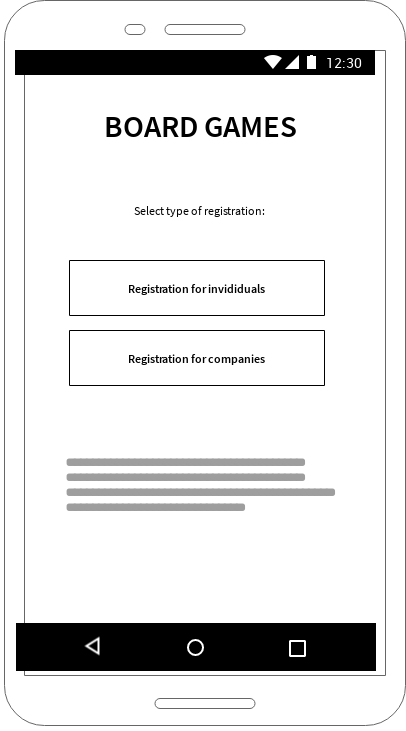
\includegraphics[scale=0.9]{img/entrance_window}
	\caption{Langas, rodomas atidarius programėlę}
	\label{img:entrance_window}
\end{figure}

\begin{figure}[H]
	\centering
	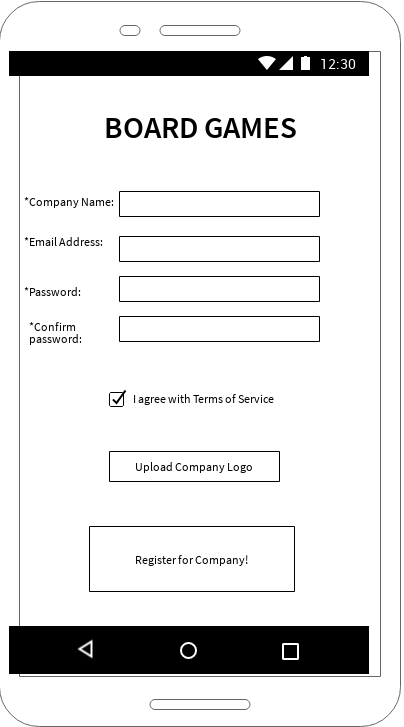
\includegraphics[scale=0.9]{img/company_register}
	\caption{Naujos kompanijos registracijos langas}
	\label{img:company_register}
\end{figure}

\begin{figure}[H]
	\centering
	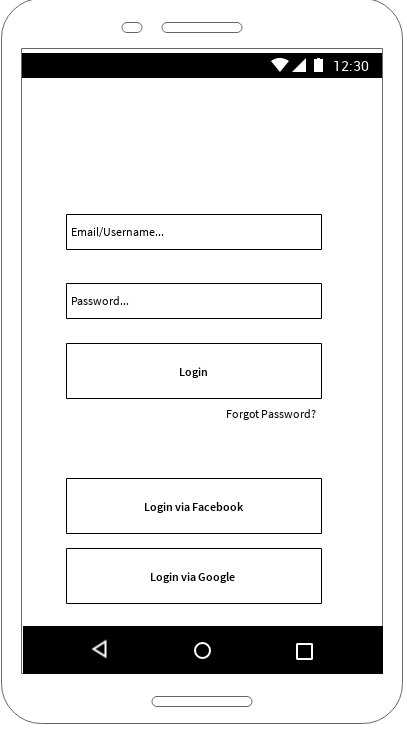
\includegraphics[scale=0.9]{img/login_window}
	\caption{Prisijungimo langas}
	\label{img:login_window}
\end{figure}

\begin{figure}[H]
	\centering
	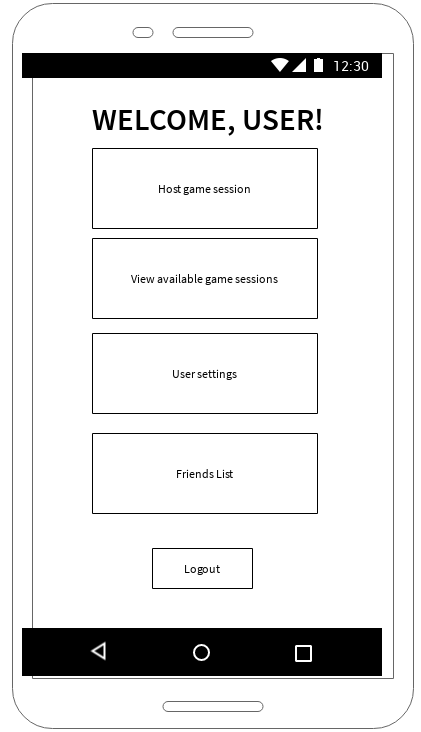
\includegraphics[scale=0.9]{img/main_window}
	\caption{Pagrindinis langas}
	\label{img:main_window}
\end{figure}

\begin{figure}[H]
	\centering
	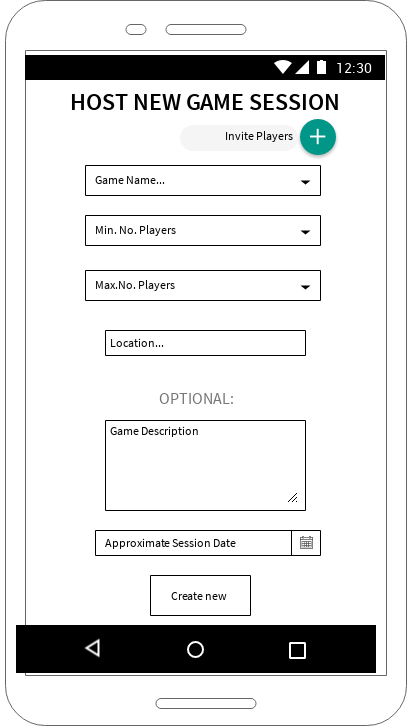
\includegraphics[scale=0.9]{img/host_game_window}
	\caption{Žaidimo kūrimo langas}
	\label{img:host_game_window}
\end{figure}

\begin{figure}[H]
	\centering
	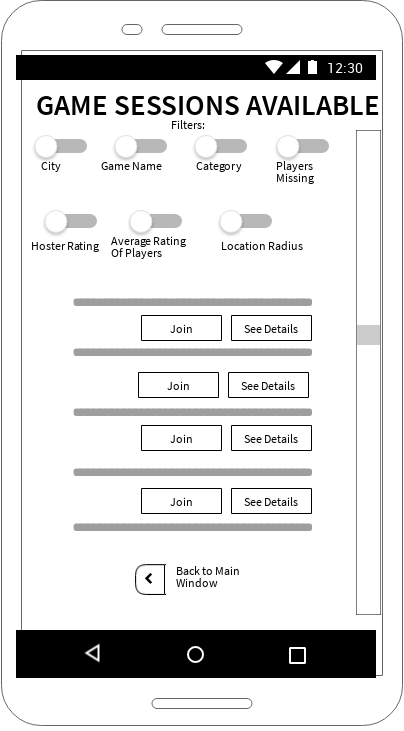
\includegraphics[scale=0.9]{img/game_sessions_view}
	\caption{Žaidimų pasirinkimo langas}
	\label{img:game_sessions_view}
\end{figure}

\sectionnonum{Rezultatas}
Dokumente detaliai apibrėžti mobiliosios stalo žaidimų programėlės architektūros funkciniai reikalavimai iš asmeninio vartotojo, kompanijos, administracijos perspektyvos, taip pat nefunkciniai, vartotojo sąsajos reikalavimai. Pagal užsakovo poreikius išskirtos dvi vartotojų kategorijos - paprasti vartotojai, žaidžiantys stalo žaidimus ir stalo žaidimų kūrimo kompanijos, pranešančios naujienas, organizuojančios konkursus, matančios stalo žaidimų sesijų visumos statistiką. Taip pat dokumento priede pateikti numatomos sistemos vartotojo sąsajos brėžiniai, leidžiantys geriau suvokti numatomas sistemos sąsajos galimybes.

\sectionnonum{Išvada}
Apibrėžtų stalo žaidimų programėlės architektūros reikalavimų visuma leidžia vykdyti tolimesnį etapą - konkrečios sistemos kūrimo darbus, pasitelkiant IT architektus ir programuotojus. Sukurtų reikalavimų sėkmės požymis - dokumentas vienareikšmiškai vienodai suvokiamas tiek verslo aplinkos žmonių, tiek ir IT srities atstovų.

\sectionnonum{Literatūros sąrašas}
\begin{itemize}
	\item Doc. dr. K. Petrausko Programų Sistemų Inžinerijos kurso konspektai
    \item A. Abran, J. W. Moore, P.Bourque, R. Dupuis, L. L. Tripp - ,,Guide to the Software Engineering Body of Knowledge''
	\item UML dokumentacija \url{https://www.tutorialspoint.com/uml/uml_2_overview.htm}
	\item OMG UML v.2.5 Dokumentacija diagramoms, žymėjimui
\end{itemize}

\end{document}


